\documentclass{article}

\usepackage{graphicx}
\usepackage{tikz}
\usepackage{tikzsymbols}
\usetikzlibrary{calc,patterns,shapes.geometric}
\pagestyle{empty}
\usepackage[margin=0pt]{geometry}
\geometry{papersize={14in,12in}}

\def\centerarc[#1](#2)(#3:#4:#5){\draw[#1] ($(#2)+({#5*cos(#3)},{#5*sin(#3)})$) arc (#3:#4:#5);}

\begin{document}
	\begin{figure}
		\centering
		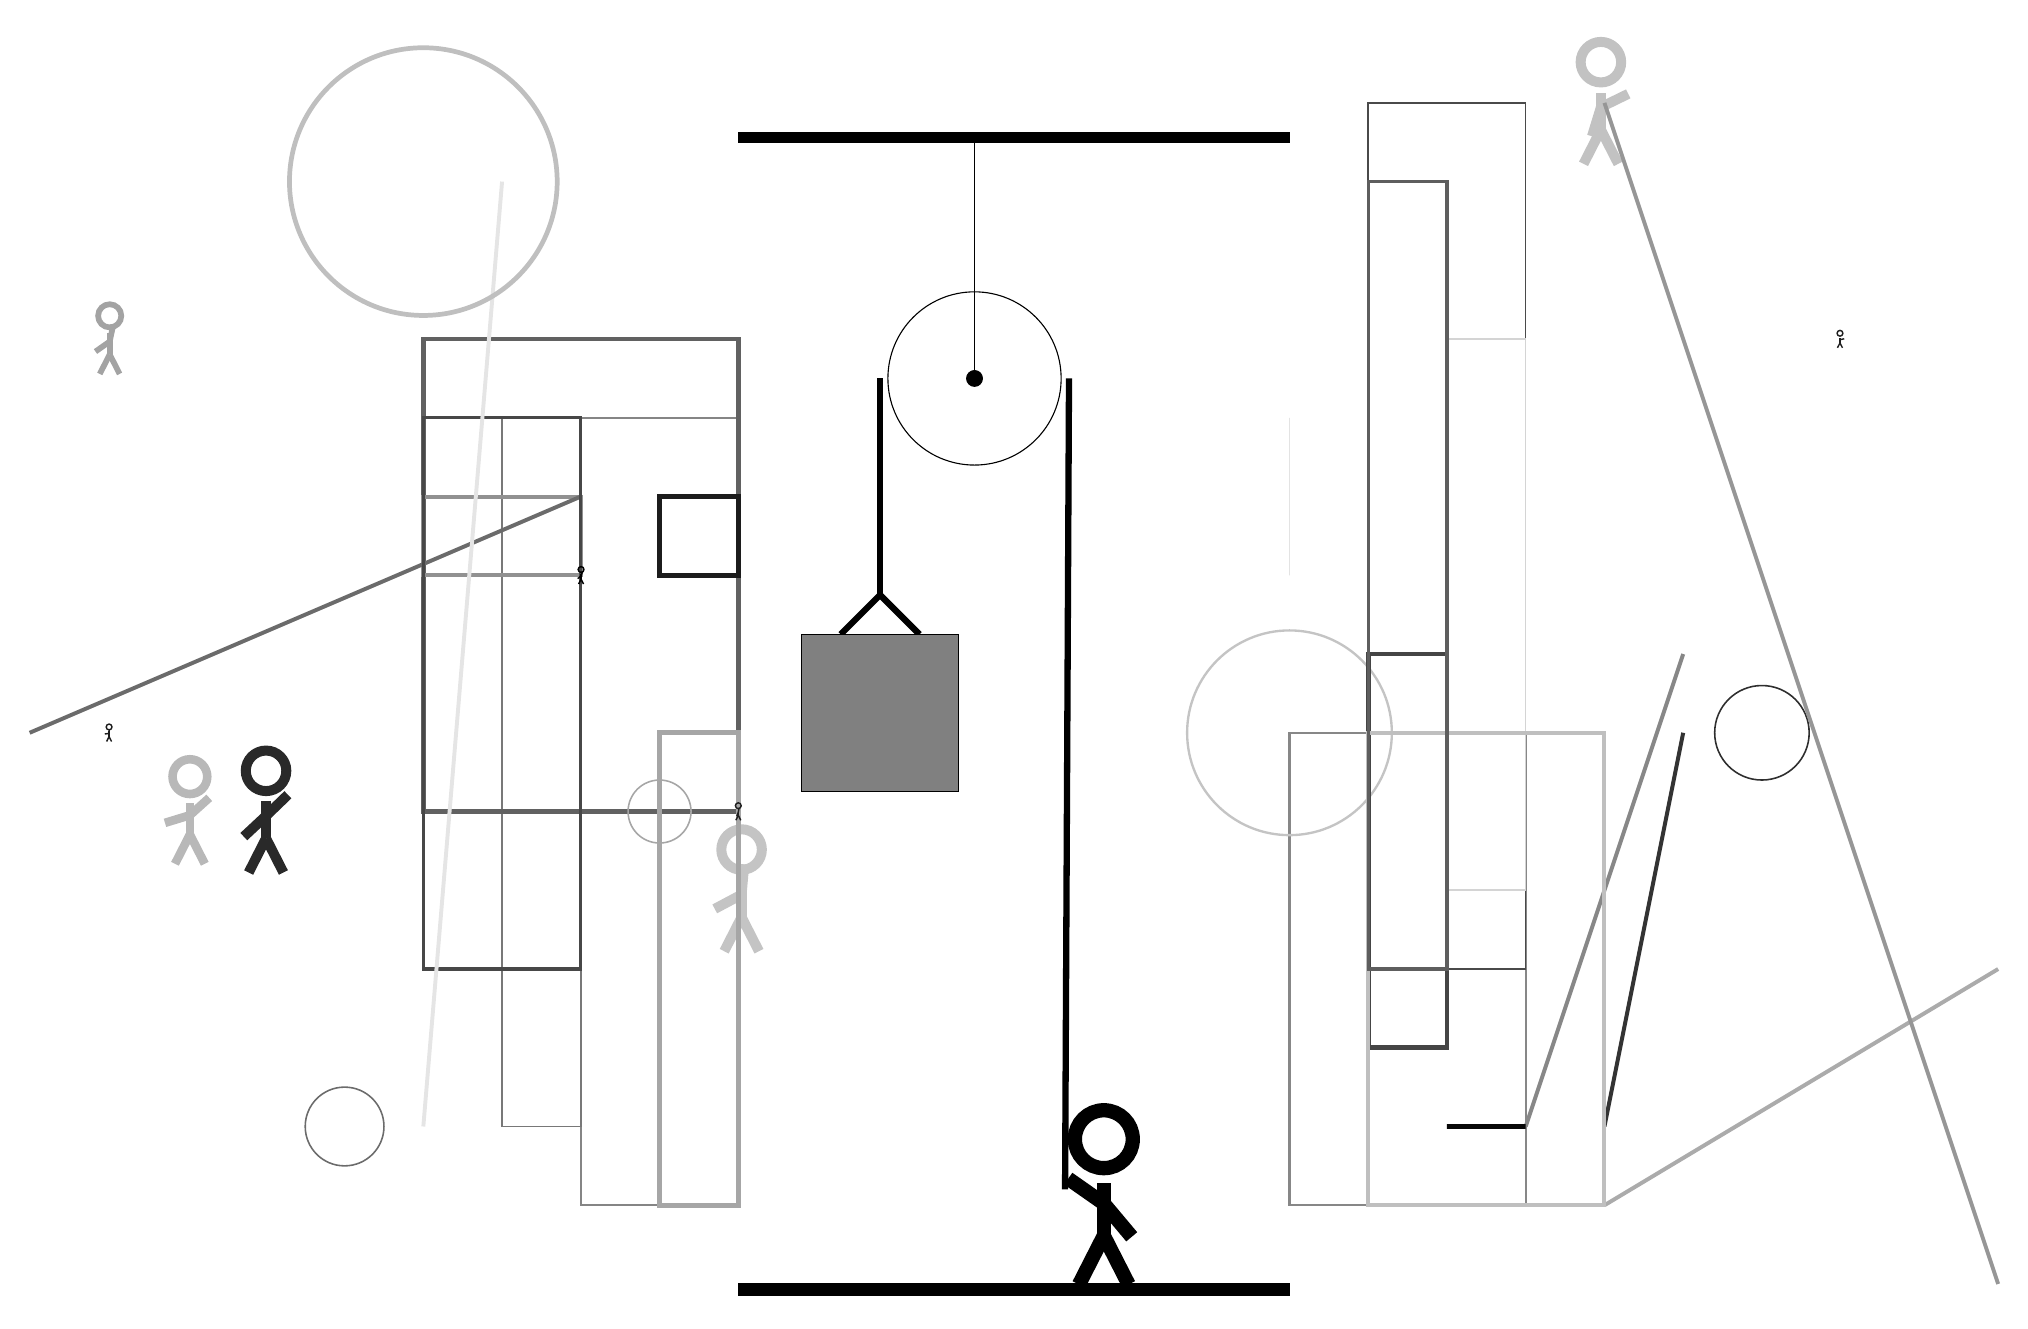
\begin{tikzpicture}
			%%%%% START %%%%%
			
			\draw[fill=black] (-2, 11.5) rectangle (5, 11.625);
			
			\draw (1, 8.5) circle (1.1);
			\draw[fill=black] (1, 8.5) circle (0.1);
			\draw (1, 11.5) -- (1, 8.5);
			
			\draw[line width=0.8mm] (-0.7, 5.25) -- (-0.2, 5.75) -- (0.3, 5.25);
			\draw[fill=black!50] (-1.2, 5.25) rectangle (0.8, 3.25);
			
			\draw[line width=0.3mm, color=black!48] (-4, 8) rectangle (-2, -2);
			
			\draw[line width=0.5mm, color=black!33](9, -2) -- (14, 1);
			\draw[line width=0.3mm, color=black!47] (5, 4) rectangle (8, -2);
			\draw[line width=0.2mm, color=black!53] (-4, -1) rectangle (-5, 8);
			
			\node[line width=0.4mm, color=black!36] at (-10, 9) {\Strichmaxerl[4][35][78]};
			
			\node[line width=0.4mm, color=black!24] at (9, 12) {\Strichmaxerl[7][73][26]};
			\node[line width=0.2mm, color=black!23] at (-2, 2) {\Strichmaxerl[7][28][85]};
			\draw[line width=0.6mm, color=black!62] (-2, 3) rectangle (-6, 9);
			\node[line width=0.7mm, color=black!89] at (-10, 4) {\Strichmaxerl[1][8][87]};
			\draw[line width=0.2mm, color=black!71] (6, 12) rectangle (8, 1);
			
			\draw[line width=0.5mm, color=black!43] (-4, 7) rectangle (-6, 6);
			\draw[line width=0.5mm, color=black!80](9, -1) -- (10, 4);
			\draw [line width=0.2mm, color=black!58](-7, -1) circle (0.5);
			
			\draw[line width=0.5mm, color=black!58](-4, 7) -- (-11, 4);
			\draw[line width=0.2mm, color=black!11] (5, 8) rectangle (5, 6);
			\node[line width=0.4mm, color=black!88] at (12, 9) {\Strichmaxerl[1][89][12]};
			
			\draw[line width=0.4mm, color=black!72] (-4, 8) rectangle (-6, 1);
			\draw[line width=0.6mm, color=black!35] (-3, -2) rectangle (-2, 4);
			\draw[line width=0.5mm, color=black!10](-5, 11) -- (-6, -1);
			\draw [line width=0.3mm, color=black!23](5, 4) circle (1.3);
			\draw[line width=0.6mm, color=black!73] (7, 5) rectangle (6, 0);
			
			\draw [line width=0.6mm, color=black!25](-6, 11) circle (1.7);
			\draw[line width=0.7mm, color=black!89] (-3, 7) rectangle (-2, 6);
			\draw[line width=0.2mm, color=black!17] (7, 9) rectangle (8, 2);
			\node[line width=0.5mm, color=black!28] at (-9, 3) {\Strichmaxerl[6][17][42]};
			\draw[line width=0.5mm, color=black!47](10, 5) -- (8, -1);
			\node[line width=0.3mm, color=black!84] at (-8, 3) {\Strichmaxerl[7][43][44]};
			\draw [line width=0.2mm, color=black!82](11, 4) circle (0.6);
			\draw[line width=0.5mm, color=black!25] (6, -2) rectangle (9, 4);
			
			\draw[line width=0.5mm, color=black!41](9, 12) -- (14, -3);
			\node[line width=0.3mm, color=black!100] at (-4, 6) {\Strichmaxerl[1][39][71]};
			\node[line width=0.4mm, color=black!88] at (-2, 3) {\Strichmaxerl[1][70][79]};
			\draw[line width=0.4mm, color=black!63] (6, 1) rectangle (7, 11);
			\draw [line width=0.2mm, color=black!35](-3, 3) circle (0.4);
			\draw[line width=0.7mm, color=black!97] (7, -1) rectangle (8, -1);
			
			\draw[line width=0.8mm] (-0.2, 8.5) -- (-0.2, 5.75);
			\centerarc[line width=0.8mm](1, 8.5)(0:180:1.2000000000000002);
			\draw[line width=0.8mm](2.2, 8.5) -- (2.15, -1.8);
			
			\node at (2.6, -1.9) {\Strichmaxerl[10][-35][-50]};
			
			\draw[fill=black] (-2, -3) rectangle (5, -3.15);
			
			%%%%% END %%%%%
		\end{tikzpicture}
	\end{figure}	
\end{document}